\chapter{Overall system design}
The purpose of this chapter is to give an outline of the design ideas considered for the system. As the problem statement pointed out, the system will consist of a processing system which will allow for adjustment when in use, such that the speaker will not suffer from the voice coil hitting the backplate. As shown in \autoref{fig:speaker_block2} the system will be integrated within an active speaker where it will act as the processing system between the external audio source and the amplifier.

\begin{figure}[H]
	\centering
	\tikzsetnextfilename{SpeakerBlock}
	\scalebox{0.9}{
		\begin{tikzpicture}
%% Audio Source %%
\node [block, fill=white] (AudioSource) at (0,0) {Audio Source};

%% Subsystems in enclosure %%
\node [block, fill=white] (Signal processor) at ($(AudioSource)+(4,0)$) {Signal processor};
\node [block, fill=white] (Amplifier) at ($(Signal processor)+(4,0)$) {Amplifier};
\node [block, fill=white] (PSU) at ($(Amplifier)+(0,2)$) {PSU};
\node [block, fill=white] (Driver) at ($(Amplifier)+(3.5,0)$) {Driver};

%% Store Blokke %%
\begin{pgfonlayer}{bg}
\draw[thick, fill=black!20] ($(-6,3)+(Amplifier)$) -- ($(1.750,3)+(Driver)$) -- ($(1.750,-1.25)+(Driver)$) -- ($(-6,-1.25)+(Amplifier)$) -- ($(-6,3)+(Amplifier)$); 
\node (Speakertag) at ($(-.25,-1)+(Driver)$) {\textbf{Speaker Enclosure}};
\end{pgfonlayer}

%% Forbindelse %%
\draw[->,thick] (AudioSource) -- (Signal processor);
\draw[->,thick] (PSU) -- (Amplifier);
\draw[->,thick] (Signal processor) -- (Amplifier);
\draw[->,thick] (Amplifier) -- (Driver);
\draw[->, to path={-| (\tikztotarget)},thick] (PSU) edge (Signal processor);
%\draw[->] ($(EnclosureDriver)+(-1.375,0.3)$) -- ($(EnclosureDriver)+(-1.75,0.3)$) -- ($(EnclosureDriver)+(-1.75,1)$) -- ($(EnclosureDriver)+(-5.5,1)$) |- ($(SpectralAnalysis)+(1.375,0.3)$);

\end{tikzpicture}}
	\caption{Block diagram of an active speaker.}
	\label{fig:speaker_block2}
\end{figure}


%\begin{figure}[H]
%\centering
%\tikzsetnextfilename{SpeakerBlock2}
%\scalebox{0.9}{
%\begin{tikzpicture}
%% Audio Source %%
\node [block, fill=black!80,text=white] (AudioSource) at (0,0) {Audio Source};

%% Subsystems in enclosure %%
\node [block, fill=blue!15] (Signal processing system) at ($(AudioSource)+(4,0)$) {Processing system};
\node [block, fill=black!80,text=white] (Amplifier) at ($(Signal processing system)+(4,0)$) {Amplifier};
\node [block, fill=black!80,text=white] (PSU) at ($(Amplifier)+(0,2)$) {PSU};
\node [block, fill=black!80,text=white] (Driver) at ($(Amplifier)+(3.5,0)$) {Driver};

%% Store Blokke %%
\begin{pgfonlayer}{bg}
\draw[thick, fill=black!10] ($(-6.2,3)+(Amplifier)$) -- ($(1.750,3)+(Driver)$) -- ($(1.750,-1.25)+(Driver)$) -- ($(-6.2,-1.25)+(Amplifier)$) -- ($(-6.2,3)+(Amplifier)$); 
\node (Speakertag) at ($(-.25,-1)+(Driver)$) {\textbf{Speaker Enclosure}};
\end{pgfonlayer}

%% Forbindelse %%
\draw[->,thick] (AudioSource) -- (Signal processing system);
\draw[->,thick] (PSU) -- (Amplifier);
\draw[->,thick] (Signal processing system) -- (Amplifier);
\draw[->,thick] (Amplifier) -- (Driver);
\draw[->, to path={-| (\tikztotarget)},thick] (PSU) edge (Signal processing system);
%\draw[->] ($(EnclosureDriver)+(-1.375,0.3)$) -- ($(EnclosureDriver)+(-1.75,0.3)$) -- ($(EnclosureDriver)+(-1.75,1)$) -- ($(EnclosureDriver)+(-5.5,1)$) |- ($(SpectralAnalysis)+(1.375,0.3)$);

\end{tikzpicture}}
%\caption{Block diagram of an active speaker.}
%\label{fig:speaker_block2}
%\end{figure}

The starting point of the design concept is to determine what type of processing system is going to be developed. Different plausible solution will be reviewed and evaluated in order to determine what solutions would be optimally. 


\section{Analogue versus digital}
It is important to clarify if the processing system is going to be designed as an analogue or digital system. Both types have its own advantages and disadvantages and one of the purposes of this section is thus to determine which platform will suit the system most. A brief analysis on the advantages and disadvantages of both system are therefore provided. 

The main difference between an analogue and digital system is that the analogue system works in continuous-time while the digital system works in discrete-time. For a analogue system values of a continuous signal, at any given time, is defined. For a digital system, values of a signal are only defined at specific points in time with a fixed resolution. The time difference between each points is defined through defined sampling period $T_s$ and the resolution of each point is defined by the resolution of the Analogue-to-Digital Converter (ADC). By using a digital system, some information of the signal may be lost, since there will be points in time where the signal is not defined, a problem known as quantization.

For an analogue system, components such as resistors, capacitors, inductors, transistors and so on, are usually used. A digital system will typically consist of an ADC to discretize the analogue signal, a processor to process the signal, and a Digital-to-Analogue Converter (DAC) to convert the signal back to an continuous signal. The advantage of designing an analogue system is that ideally no information is lost. Assuming that the analogue components are ideal since distortion will arise as soon as non-ideal components are used. The problem with ideal components are not a problem in digital system, since no further distortion will be applied to the signal as soon as the signal is made discrete. The main disadvantages of the digital system lies in the conversion where quantization noise could arise as a problem if the resolution of the conversion is not high enough. 

As the system to be developed, most likely will rely on signal processing, the great disadvantages of an analogue system is the constraints and flexibility to apply signal processing compared to a digital system. Some applications such as the Fourier Transformation is very hard if not impossible to realize in an analogue system while realizable in a digital system through algorithms. Also, if the system is large, an analogue system might turn out to be very complex.%, and use more components which results in more distortion. 
As the system to be developed is relying on signal processing the platform is chosen to be digital.

\subsection{Real-time System} \label{sec:RealTime}
Because a digital system is going to be used the question arises of using real-time or none real time. It diverges again in advantages and disadvantages of both systems. %A brief overview will be given which will be used to support the chosen system.

\subsubsection*{Real-time}
A real time system offers it advantages that when in use it can work continuously with the given input and possible adapt to the given situation. This increases the flexibility of the system because adjustment can be done in real time and therefore detect problems and possibly avoid a bad outcome. 
%\textbf{The real time system can easily be adapted into other system because the algorithm has not changed and only need new parameters.} 
The system would be able to function when needed for the user, which is important when in e.g. music applications. There is only one big disadvantage of the real time system. Based on the frequency range of the signal the system works with, the real time system should be able to do all the needed calculation before the next sample. This limits the system to a certain amount of time and specific algorithms like large point FFT´s or division. %With a certain time given it might not be possible to finish the needed calculation and if that happens, the system will fail.

\subsubsection*{None real-time}
The none real time system has the advantage of all the time it needs. Since it is not made for running in the specific situation it can perform rather complex calculation and not worry about how many iterations it might need. This means that low cost system can be used since computational power is not a problem. The system would be able to consider possible outcomes and generate a perfectly adjusted signal. Considering those advantages the major drawback is that is does not function when the user might need the functions. The none real-time would need time which might not be desirable. A situation could be when listening to music where a loading time of larger proportions are not acceptable 

Due to the fact that the system revolves around a active speaker system and is going to handle music signals it seems most fit to use a real-time system. This gives the most flexibility and pleases the end user by not having to wait for analysis of the signal.




%% Feedback vs Feed Forward %%
\section{Real-time Signal Processing System}

It is important to clarify if the processing system is going to be designed as an analog or digital system. Both types have its own advantages and disadvantages and one of the purposes of this section is thus to determine which platform will suit the system most. A brief analysis on the advantages and disadvantages of both system are therefore provided. 

Briefly, the main difference between an analog and digital system is that the analog system works in continuous-time while the digital system works in discrete-time. For a continuous-time system values of a continuous signal, at any given time, is defined. For a discrete-time system, values of a signal are only defined at specific points in time with a fixed resolution. The time difference between each points is defined through defined sampling period $T_s$ and the resolution of each point is defined by the resolution of the Analog-to-Digital Converter (ADC). By using a digital system, some information of the signal is necessarily lost, since there will be points in time where the signal is not defined.

For an analog system, components such as resistors, capacitors, inductors, transistors and so on, are usually used. A digital system will typically consist of an ADC to discretize the analog signal, a processor to process the signal, and a Digital-to-Analog Converter (DAC) to convert the signal back to an analog signal. The advantage of designing an analog system is that ideally no information is lost. This conclusion is however derived with the assumption that analog components are ideal since distortion will arise as soon as non-ideal components are used. The problem with ideal components is not a problem for a digital system, since no further distortion will be applied to the signal as soon as the signal is discretized.

As the system to be developed, most likely will rely on signal processing, the great disadvantages of an analog system is the constraints and flexibility to apply signal processing compared to a digital system. Some applications such as the Fourier Transformation is very hard if not impossible to realize in an analog system while realizable in a digital system through algorithms. Also, if the system is large, an analog system might turn out to be very complex, and use more components which results in more distortion. As the system to be developed is relying on signal processing the platform is chosen to be digital.

\section{Feedback versus Feedforward System} \label{sec:feedback}

At this point it is yet to be determined if the system will be based on a feedback or a feedforward system. The choices are to design a feedback system that will decide what to do, based on real-time measurements from a sensor i.e. accelerometer, or a feedforward system that will analyse an input signal and then decide what to do. Previous tests have shown that it is possible to use an accelerometer to estimate the performance of the system by looking at the harmonic distortions. A big issue is to analyse harmonic distortions when music is played back, as estimating harmonic distortions introduced in a system, are only well-defined for periodic sinusoids. The tests of the loudspeaker also showed that the frequency response of vibration on the driver and cabinet hardly changes when exposed for loud playback, thus it will be hard to derived anything alone from the frequency response of the vibrations. It can therefore be concluded that developing a system based on measurements from a accelerometer might turn out to be too complex to be realized in time due to time constraints. The system to be designed will therefore be based on a feedforward system. The concept of a feedback system which fulfil the problem statement is shown in \autoref{fig:Concept}.

\begin{figure}[H]
\centering
\tikzsetnextfilename{Concept}
\scalebox{0.8}{
\begin{tikzpicture}
%% Kasser %%
\node [block, fill=black!80,text=white] (AudioSource) at (0,0) {Audio Source};

%% DSP %%
%\node [block, fill=blue!15] (Equalizer1) at ($(AudioSource)+(3.5,0)$) {Equalizer};
\node [block, fill=blue!15] (SpectralAnalysis) at ($(AudioSource)+(3.5,0)$) {Signal analysis};
\node [block, fill=blue!15] (Equalizer) at ($(SpectralAnalysis)+(4.5,0)$) {Signal processing};


%% External %%
%\node [block, fill=blue!15] (UserInterface) at ($(Equalizer1)+(-3.5,2)$) {User interface};
%\node [block, fill=blue!15] (UserInterfaceDev) at ($(Equalizer1)+(3.5,2)$) {Developer interface};

%% Speaker Enclosure %%
\node [block, fill=black!80,text=white] (Amplifier) at ($(SpectralAnalysis)+(4.5,-3)$) {Amplifier};
\node [block, fill=black!80,text=white] (Driver) at ($(Amplifier)+(-3.5,0)$) {Driver};

%\node (User) at ($(-2.5,0)+(UserInterface)$) {\textbf{User}};
%\node (Developer) at ($(3.6,0)+(UserInterfaceDev)$) {\textbf{Developer}};
%\draw[->] (User) -- (UserInterface);
%\draw[->] (Developer) -- (UserInterfaceDev);

% Store Blokke %%
\begin{pgfonlayer}{background}
\draw[thick, fill=black!10] ($(-1.75,1.2)+(SpectralAnalysis)$) -- ($(2.5,1.2)+(Equalizer)$) -- ($(2.5,-1.5)+(Equalizer)$) -- ($(-1.75,-1.5)+(SpectralAnalysis)$) -- ($(-1.75,1.2)+(SpectralAnalysis)$);
\node (DSPtag) at ($(1,-1.1)+(SpectralAnalysis)$) {\textbf{Digital Processing System}};

\draw[thick, fill=black!10] ($(-2.5,1)+(Driver)$) -- ($(2.5,1)+(Amplifier)$) -- ($(2.5,-1.5)+(Amplifier)$) -- ($(-2.5,-1.5)+(Driver)$) -- ($(-2.5,1)+(Driver)$);
\node (DSPtag) at ($(2,-1.1)+(Driver)$) {\textbf{Speaker Enclosure}};
\end{pgfonlayer}

%% Forbindelse %%
\draw[->] (AudioSource) -- (SpectralAnalysis);
%\draw[->] (Equalizer1) -- (SpectralAnalysis);
\draw[->] (SpectralAnalysis) -- (Equalizer);
\draw[->] (Equalizer) -- (Amplifier);
\draw[->] (Amplifier) -- (Driver);

%\draw[->] (UserInterface) -| ($(Equalizer1)+(-.25,.6)$);
%\draw[->] (UserInterfaceDev) -| ($(Equalizer1)+(.25,.6)$);

%\draw[->] ($(SensorDriver)+(-1.375,-0.3)$) -- ($(SpectralAnalysis)+(1.375,-0.3)$);

%\draw[->] (SpectralAnalysis) -- (Decisionblock);
%\draw[->] (Decisionblock) |- (Equalizer);
\end{tikzpicture}}
\caption{Overview of design concept.}
\label{fig:Concept}
\end{figure}

The design concept consist of a signal processing block, which will be analysed to understand which solution is best for the problem stated, a signal analysis block which will not be analysed further in this chapter, a user interface which will be analysed to determine how the user interface should be designed and lastly the processor block which will be analysed to determine which type of processor that should be used. 


\subsection{Distortion from vibration and impulses}\label{subsec:impulses}

A common problem when designing loudspeakers are the vibrations from the enclosure. If the vibrations are strong, they will become audible and distort the overall sound. The sound radiation from the enclosure will become greater when the \gls{SPL} from the speaker increase. This problem is solved with different techniques but yield more or less the same outcome, which is stiffening of the enclosure. Some of the techniques for removing vibrations from the enclosure could be:
\begin{itemize}
\item Mechanical decoupling of the drivers from the enclosure.
\item Denser or heavier construction material with a high natural frequency, making it harder for the enclosure to start vibrating.
\item Dampening material or complex structural design inside the cabinet to disperse the sound.
\end{itemize}
\todo[inline]{Skal nok lige skaffe nogle kilder på de udtagelser}

Another possibility is to use the vibration measurement as an indicator to tell the current performance of the loudspeaker. Since the loudspeaker will vibrate more at higher volumes. 


Looking further into the woofer itself, it shows in \autoref{fig:SpeakerModelStress} that parts in the woofer also creates unwanted vibrations. The purpose of the woofer is to reproduce the electrical signal as an acoustical signal. This is done by using a diaphragm which is suspended in a very light and easy to move material. An Induction in the coil is created in a permanent magnet creating a a electro magnetic force resulting in the diaphragm moving. The goal will always be to loose as little as possible energy, giving the most perfect output. The woofer simply needs to be as powerful, light, stiff and efficient as possible.

\begin{figure}[H]
\centering
\begin{subfigure}[t]{0.47\textwidth}
\includegraphics[width=\linewidth]{SpeakerGOOD}
	\caption{Regular speaker driver showing surround, diaphragm and the magnet.}
	\label{fig:regularspeaker}
\end{subfigure}
\hspace{6mm} 
\begin{subfigure}[t]{0.47\textwidth}
\includegraphics[width=\linewidth]{SpeakerBAD}
	\caption{Regular speaker driver with red markings showing stress areas}
	\label{fig:badspeaker}
\end{subfigure}
\caption{A Speaker driver, where \ref{fig:badspeaker} shows the stress points outlined with red.}
\label{fig:SpeakerModelStress}
\end{figure}
%When this signal has a large amplitude, read overload, the diaphragm reaches physical capacity. 
In \autoref{fig:badspeaker} it shows that when a diaphragm is pushed to its maximum capacity the surround will affect the diaphragm causing unwanted distortion. This will be one of the major problems if the diaphragm is not sufficiently stiff to withstand the high \gls{SPL} and not twist during playback. 








%As the audio signal must be continuous when played on loudspeakers


%% Krav til Platform %%
\section{Processor Platform}
This section will reference the demands for the processor platform given by DALI and analyse which processor platform will be optimal for these condition. 

\subsection*{Demands for the platform}
The demands for the processor platform have been derived in a mail corresodance with DALI 
\todo[inline]{Reference til CD}

\textbf{Sample rate} \\
The system must be able to handle 96 kHz sample rate since peripheral components will interface be running at this rate.

\textbf{Bit resolution} \\
There must be support for audio in at least a 24 bit resolution since the \gls{DAC} chosen by DALI is of 24 bit.

\textbf{\gls{SNR}} \\
A minimum \gls{SNR} of 120 dB on the \gls{DAC} must be achieved. This will provide headroom for digital volume control.

\textbf{Instructions pr. sample.} \\
The processor must a least be able to run 1024 intructions pr. sample. which would give approximately 100 \gls{MIPS}


\textbf{Memory for both an equalizer and multi band limiter} \\
The platform will consist of an equalizer and limiter when finished. This project will however focus on the equalizer and sensory system. Hence it only desireable to leave TBD room for an multi band limiter which is desired by DALI. 


\textbf{Interfacing} \\
The platform must be able to interface with an ADC and DAC with the bus type \gls{I2S}. Besides the interfacing with the ADC and DAC the platform must be able to interface with the chosen sensor in \autoref{sec:Sensor}.

The 32 bit resolution is prefered by DALI over a 24 bit resolution because it would give a increased \gls{SNR} of 48 dB. These demands lead to the analyzation of which platform would be the most optimal.   

\subsection*{Choice of processor platform}
For the choice of processor platform different types of platforms could be used, such as a microcontroller or a \gls{DSP}. These two types of processors have different advantage and disadvantages which needs to be analyzed to find the most optimal platform for the demands above.

The basic difference between a microcontroller and a \gls{DSP} is that the \gls{DSP} is designed for fast calculating and moving data while the microcontroller is designed to be more flexible in its use and have more features.

Because the need for filtering in an equalizer is needed and the high performance demands from above the natural choice of platform would be a \gls{DSP} without further consideration.     







%% GUI %%
%\section{Graphical User Interface} \label{sec:user_interface}

Here a GUI will be developed and shit will get really crazy with C\#

%In this section an analyzation of the user interface for the equalizer analyzed in \autoref{sec:tech_equalizer} will be made to determine which user interface will be the most optimal for the specific user of the equalizer. 
%
%There are two different intended users for the equalizer: 
%\begin{itemize}
%\item The developer.
%\item The commercial user.
%\end{itemize}
%This means that there are different requirements for the specific user of the equalizer.
%
%\subsection{User interface for the developer}
%The developer is the user which knows everything about an equalizer and its effects on a system therefore the developer desires a great deal of control and options in the interface of the equalizer. This means that the interface can be complex and must not set no restrictions for the developer.  
%
%Because the developer needs to have full control of the equalizer he needs to have control of: 
%\begin{itemize}
%\item Center frequency.
%\item Q - value.
%\item Gain.
%\item Band selection.
%\end{itemize} 
%This leads to a suggestions for a user interface which gives full control to a developer.
%
%\begin{figure}[H]
%\centering
%\tikzsetnextfilename{InterfaceDev1}
%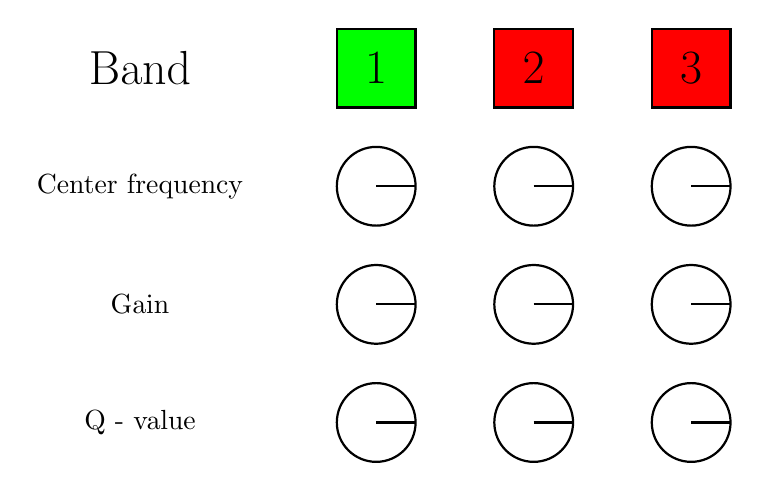
\begin{tikzpicture}
\draw[thick] (2,0) circle [radius=0.5] node at (-1,-0) {Q - value};
\draw[thick] (2,1.5) circle [radius=0.5] node at (-1,1.5) {Gain};
\draw[thick] (2,3) circle [radius=0.5] node at (-1,3) {Center frequency};
\draw node at (-1,4.5)[font=\LARGE]{Band};
\draw[thick][fill=green, draw=black](1.5,4) rectangle(2.5,5) node at (2,4.5)[font=\LARGE]{1};

\draw[thick] (4,0) circle [radius=0.5];
\draw[thick] (4,1.5) circle [radius=0.5];
\draw[thick] (4,3) circle [radius=0.5];
\draw[thick][fill=red, draw=black](1.5+2,4) rectangle(2.5+2,5) node at (2+2,4.5)[font=\LARGE]{2};

\draw[thick] (6,0) circle [radius=0.5];
\draw[thick] (6,1.5) circle [radius=0.5];
\draw[thick] (6,3) circle [radius=0.5];
\draw[thick][fill=red, draw=black](1.5+4,4) rectangle(2.5+4,5) node at (2+4,4.5)[font=\LARGE]{3};

\draw[thick](6,0) -- (6.5,0);
\draw[thick](6,1.5) -- (6.5,1.5);
\draw[thick](6,3) -- (6.5,3);

\draw[thick](4,0) -- (4.5,0);
\draw[thick](4,1.5) -- (4.5,1.5);
\draw[thick](4,3) -- (4.5,3);

\draw[thick](2,0) -- (2.5,0);
\draw[thick](2,1.5) -- (2.5,1.5);
\draw[thick](2,3) -- (2.5,3);
\end{tikzpicture}
%\caption{Developer user interface.}
%\label{fig:Dev_sug}
%\end{figure}
%
%The suggestion on \autoref{fig:Dev_sug} has push buttons on the bands so they can be toggled on and of while the center frequency, gain and Q - value for each band can be changed with the use of knobs. The suggestion will be accompanied by a big screen where the frequency response of the equalizer can be seen. 
%
%\subsection{User interface for the commercial user}
%The commercial user is the user which knows the implication of different the different settings of an equalizer but does not know anything about the technical aspect of an equalizer. This means that the interface needs to be simple and show what implpication a setting has on a system but leave out all technical aspects. 
%
%Because the commercial user only needs presets like for example "rock", "jazz" and "movie" the user only needs to have control of: 
%\begin{itemize}
%\item Presets.
%\end{itemize} 
%This leads to some different suggestions for a user interface which consist of a few buttons to keep it as simple as possible.
%
%
%\begin{figure}[H]
%\centering
%\begin{subfigure}[t]{0.47\textwidth}
%	\centering
%	\tikzsetnextfilename{InterfaceUser1}
%	\scalebox{0.2}{
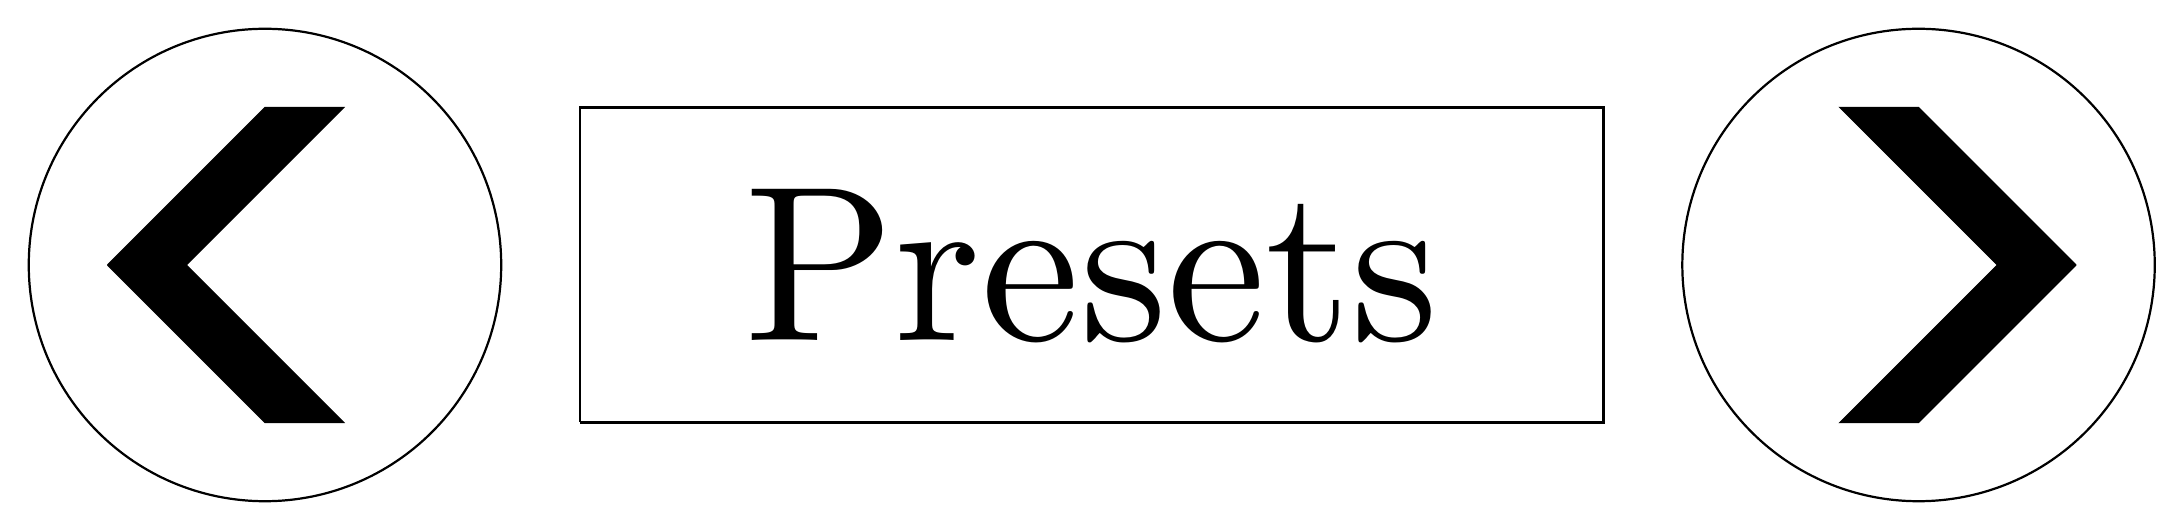
\begin{tikzpicture}
\draw [thick](-10,6) circle [radius=3];
\draw [thick](11,6) circle [radius=3];
\draw [thick](-6,4) -- (7,4) -- (7,8) -- (-6,8) -- (-6,4);
\draw[fill] (-12,6) -- (-10,8) -- (-9,8) -- (-11,6) -- (-9,4) -- (-10,4) -- (-12,6);
\draw[fill](13,6) -- (11,8) -- (10,8) -- (12,6) -- (10,4) -- (11,4)--(13,6) ;
\node[scale=8.0] (c) at (0.5,6) {Presets};
\end{tikzpicture}}
%	\caption{Suggestion 1}
%	\label{fig:UI_sug_1}
%\end{subfigure}
%\hspace{6mm} 
%\begin{subfigure}[t]{0.47\textwidth}
%	\centering
%	\tikzsetnextfilename{InterfaceUser2}
%	\scalebox{0.6}{
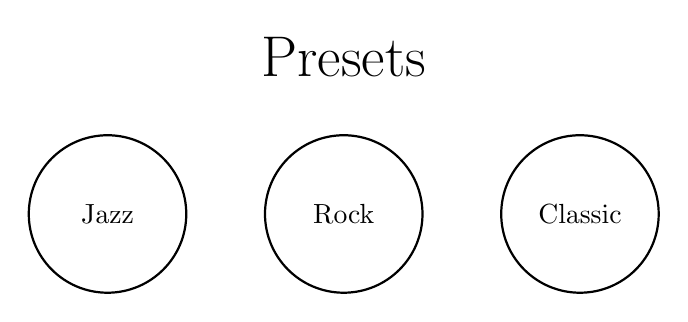
\begin{tikzpicture}
\draw [thick](0,0) circle [radius=1] node{Jazz};
\draw [thick](3,0) circle [radius=1] node{Rock};
\draw [thick](6,0) circle [radius=1] node{Classic};
\draw node at (3,2)[font=\huge]{Presets};
\end{tikzpicture}}
%	\caption{Suggestion 2}
%	\label{fig:UI_sug_2}
%\end{subfigure}
%\caption{Commercial user interface suggestions.}
%\label{fig:UI_sug}
%\end{figure}
%
%Suggestion one as seen on \autoref{fig:UI_sug_1} has two push buttons and a small screen so the user can interchange between different settings, while suggestion two has x number of push buttons which represents a preset each. The advantage of suggestion two is the overview and simplicity while suggestion one can have a larger number of presets without changing the appearance of the user interface. 
%
%The suggestions for the user interface for both the developer and the commercial user will be choosen in the requirement specification \todo[inline]{reference}  
%
